\documentclass[tikz,border=12pt]{standalone}
\usepackage[T1]{fontenc}
\usepackage[utf8]{inputenc}
\usepackage{lmodern}
\usetikzlibrary{arrows.meta}
\definecolor{purple}{HTML}{4B2BE2}
\definecolor{soft}{HTML}{F5F3FC}
\definecolor{light}{HTML}{F5F5F5}
\definecolor{edge}{HTML}{E5E5E5}
\begin{document}
\sffamily
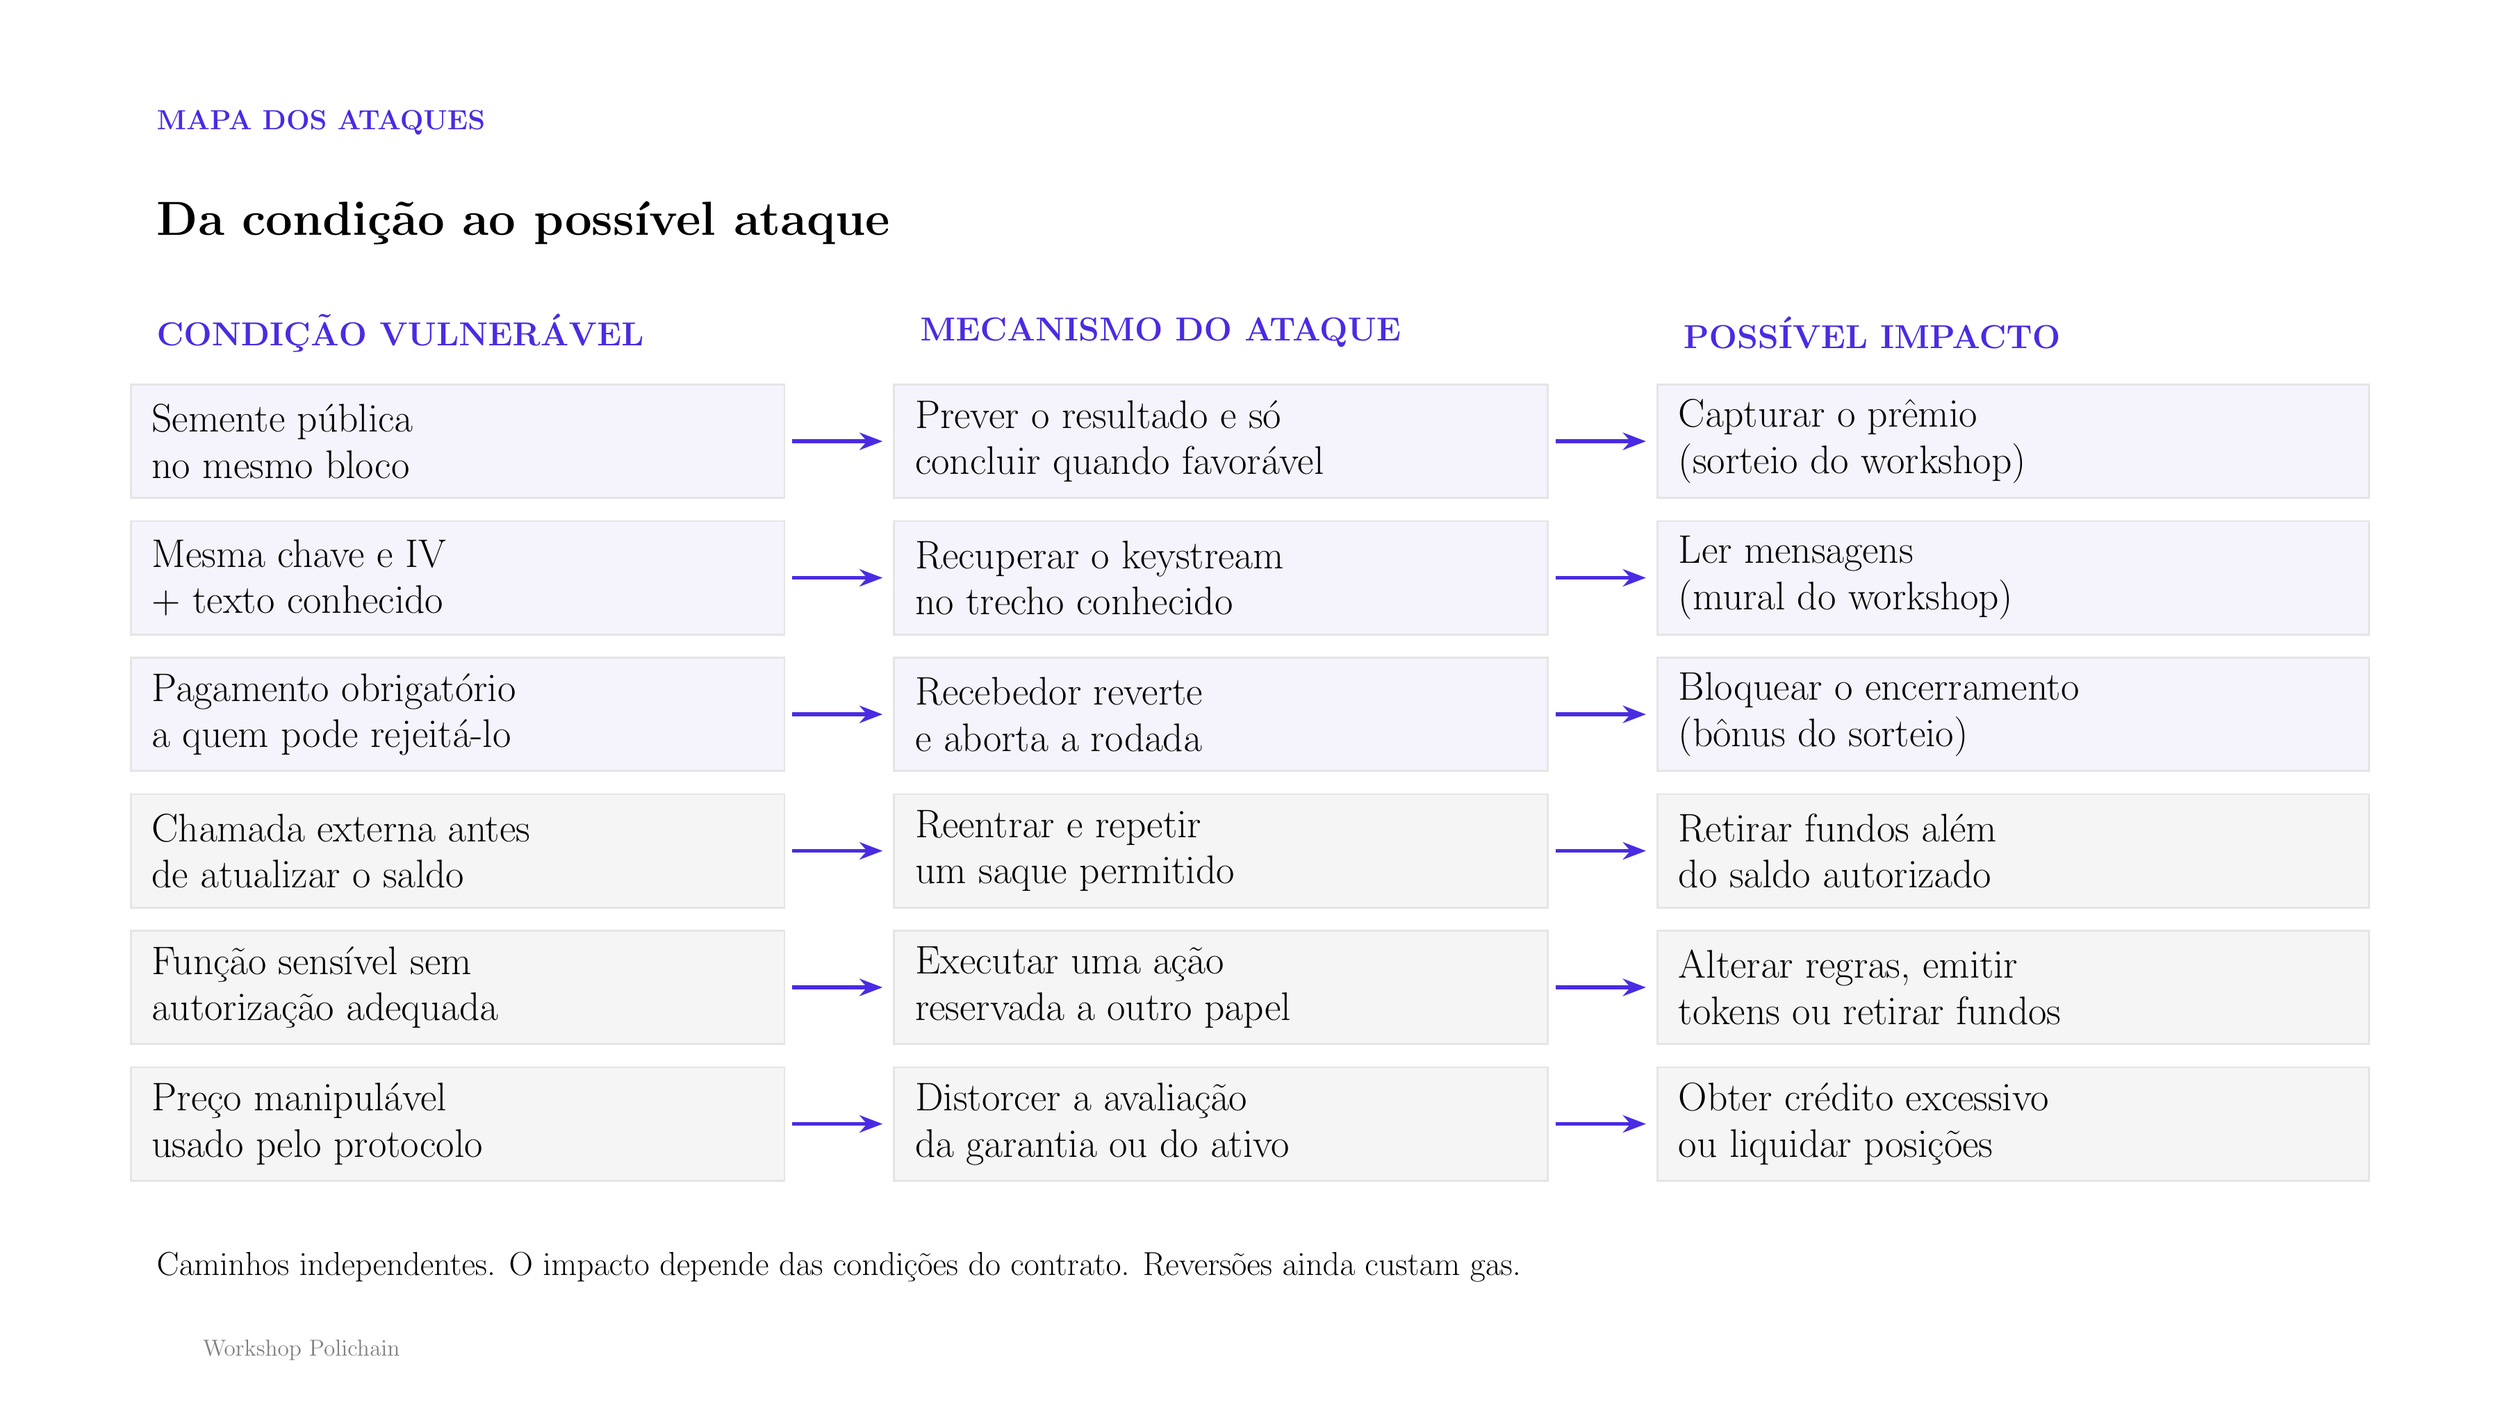
\begin{tikzpicture}[x=1pt,y=-1pt,>=Stealth]
\path[use as bounding box] (0,0) rectangle (1280,720);
\fill[white] (-12,-12) rectangle (1292,732);
\node[anchor=west,text=purple,font=\bfseries\fontsize{14}{17}\selectfont] at (68,54) {MAPA DOS ATAQUES};
\node[anchor=west,font=\bfseries\fontsize{40}{46}\selectfont] at (68,106) {Da condição ao possível ataque};
\node[anchor=west,text=purple,font=\bfseries\fontsize{16}{20}\selectfont] at (68,163) {CONDIÇÃO VULNERÁVEL};
\node[anchor=west,text=purple,font=\bfseries\fontsize{16}{20}\selectfont] at (465,163) {MECANISMO DO ATAQUE};
\node[anchor=west,text=purple,font=\bfseries\fontsize{16}{20}\selectfont] at (862,163) {POSSÍVEL IMPACTO};
\node[draw=edge,fill=soft,line width=1pt,minimum height=59pt,text width=318pt,inner xsep=11pt,align=left,font=\fontsize{20}{24}\selectfont] at (228,219.5) {Semente pública\\no mesmo bloco};
\node[draw=edge,fill=soft,line width=1pt,minimum height=59pt,text width=318pt,inner xsep=11pt,align=left,font=\fontsize{20}{24}\selectfont] at (625,219.5) {Prever o resultado e só\\concluir quando favorável};
\node[draw=edge,fill=soft,line width=1pt,minimum height=59pt,text width=348pt,inner xsep=11pt,align=left,font=\fontsize{20}{24}\selectfont] at (1037,219.5) {Capturar o prêmio\\(sorteio do workshop)};
\draw[->,purple,line width=2pt] (402,219.5) -- (449,219.5);
\draw[->,purple,line width=2pt] (799,219.5) -- (846,219.5);
\node[draw=edge,fill=soft,line width=1pt,minimum height=59pt,text width=318pt,inner xsep=11pt,align=left,font=\fontsize{20}{24}\selectfont] at (228,290.5) {Mesma chave e IV\\+ texto conhecido};
\node[draw=edge,fill=soft,line width=1pt,minimum height=59pt,text width=318pt,inner xsep=11pt,align=left,font=\fontsize{20}{24}\selectfont] at (625,290.5) {Recuperar o keystream\\no trecho conhecido};
\node[draw=edge,fill=soft,line width=1pt,minimum height=59pt,text width=348pt,inner xsep=11pt,align=left,font=\fontsize{20}{24}\selectfont] at (1037,290.5) {Ler mensagens\\(mural do workshop)};
\draw[->,purple,line width=2pt] (402,290.5) -- (449,290.5);
\draw[->,purple,line width=2pt] (799,290.5) -- (846,290.5);
\node[draw=edge,fill=soft,line width=1pt,minimum height=59pt,text width=318pt,inner xsep=11pt,align=left,font=\fontsize{20}{24}\selectfont] at (228,361.5) {Pagamento obrigatório\\a quem pode rejeitá-lo};
\node[draw=edge,fill=soft,line width=1pt,minimum height=59pt,text width=318pt,inner xsep=11pt,align=left,font=\fontsize{20}{24}\selectfont] at (625,361.5) {Recebedor reverte\\e aborta a rodada};
\node[draw=edge,fill=soft,line width=1pt,minimum height=59pt,text width=348pt,inner xsep=11pt,align=left,font=\fontsize{20}{24}\selectfont] at (1037,361.5) {Bloquear o encerramento\\(bônus do sorteio)};
\draw[->,purple,line width=2pt] (402,361.5) -- (449,361.5);
\draw[->,purple,line width=2pt] (799,361.5) -- (846,361.5);
\node[draw=edge,fill=light,line width=1pt,minimum height=59pt,text width=318pt,inner xsep=11pt,align=left,font=\fontsize{20}{24}\selectfont] at (228,432.5) {Chamada externa antes\\de atualizar o saldo};
\node[draw=edge,fill=light,line width=1pt,minimum height=59pt,text width=318pt,inner xsep=11pt,align=left,font=\fontsize{20}{24}\selectfont] at (625,432.5) {Reentrar e repetir\\um saque permitido};
\node[draw=edge,fill=light,line width=1pt,minimum height=59pt,text width=348pt,inner xsep=11pt,align=left,font=\fontsize{20}{24}\selectfont] at (1037,432.5) {Retirar fundos além\\do saldo autorizado};
\draw[->,purple,line width=2pt] (402,432.5) -- (449,432.5);
\draw[->,purple,line width=2pt] (799,432.5) -- (846,432.5);
\node[draw=edge,fill=light,line width=1pt,minimum height=59pt,text width=318pt,inner xsep=11pt,align=left,font=\fontsize{20}{24}\selectfont] at (228,503.5) {Função sensível sem\\autorização adequada};
\node[draw=edge,fill=light,line width=1pt,minimum height=59pt,text width=318pt,inner xsep=11pt,align=left,font=\fontsize{20}{24}\selectfont] at (625,503.5) {Executar uma ação\\reservada a outro papel};
\node[draw=edge,fill=light,line width=1pt,minimum height=59pt,text width=348pt,inner xsep=11pt,align=left,font=\fontsize{20}{24}\selectfont] at (1037,503.5) {Alterar regras, emitir\\tokens ou retirar fundos};
\draw[->,purple,line width=2pt] (402,503.5) -- (449,503.5);
\draw[->,purple,line width=2pt] (799,503.5) -- (846,503.5);
\node[draw=edge,fill=light,line width=1pt,minimum height=59pt,text width=318pt,inner xsep=11pt,align=left,font=\fontsize{20}{24}\selectfont] at (228,574.5) {Preço manipulável\\usado pelo protocolo};
\node[draw=edge,fill=light,line width=1pt,minimum height=59pt,text width=318pt,inner xsep=11pt,align=left,font=\fontsize{20}{24}\selectfont] at (625,574.5) {Distorcer a avaliação\\da garantia ou do ativo};
\node[draw=edge,fill=light,line width=1pt,minimum height=59pt,text width=348pt,inner xsep=11pt,align=left,font=\fontsize{20}{24}\selectfont] at (1037,574.5) {Obter crédito excessivo\\ou liquidar posições};
\draw[->,purple,line width=2pt] (402,574.5) -- (449,574.5);
\draw[->,purple,line width=2pt] (799,574.5) -- (846,574.5);
\node[anchor=west,font=\fontsize{16}{20}\selectfont] at (68,649) {Caminhos independentes. O impacto depende das condições do contrato. Reversões ainda custam gas.};
\node[anchor=west,text=gray,font=\fontsize{12}{14}\selectfont] at (92,692) {Workshop Polichain};
\end{tikzpicture}
\end{document}
